\documentclass[11pt,a4paper]{article}
\usepackage[spanish]{babel}
\usepackage[utf8]{inputenc}
\usepackage[top=2cm, bottom=2cm, left=2cm, right=2cm]{geometry}
\usepackage{lastpage,sectsty,hyperref,graphicx,pdfpages,fancyhdr,listings}

\sectionfont{\fontsize{12}{15}\selectfont}
\linespread{1.25} % Interlineado 1.5
\renewcommand{\rmdefault}{phv} % Arial
\renewcommand{\sfdefault}{phv} % Arial

\hypersetup{
    pdftitle={Trabajo Práctico 1},
	pdfsubject={Análisis Numérico I},
	pdfauthor={del Mazo Federico, Kristal Juan Ignacio},
}

\fancypagestyle{enunciado}{
    \fancyhf{}
    \fancyhead[C]{Enunciado provisto por la catedra}
}

\pagestyle{fancy}
\fancyhf{}
\fancyhead[R]{Trabajo Práctico 1 - 2018c2}
\fancyhead[L]{75.12 Análisis Numérico I}
\renewcommand{\headrulewidth}{0.4pt}
\fancyfoot[L]{100029 - 99779}
\fancyfoot[R]{\thepage de \pageref*{LastPage}}
\renewcommand{\footrulewidth}{0.4pt}
\setlength{\footskip}{17pt}

\fancypagestyle{onlyheader}{
\fancyfoot{}
}

\begin{document}

\begin{titlepage}
	\hfill
\includegraphics[width=6cm]{fiuba.jpg}
    \begin{center}
    \vfill
    \Huge \textbf{Trabajo Práctico 1}
    \vskip2cm
    \Large [75.12] Análisis Numérico I\\
    Segundo cuatrimestre de 2018
    \vfill
    \begin{tabular}{|l|c|r|}
	\hline
	Alumno & Padrón & Mail\\
	\hline
	\hline
	del Mazo, Federico & 100029 & delmazofederico@gmail.com\\
	\hline
	Kristal, Juan Ignacio & 99779 & kristaljuanignacio@gmail.com\\
	\hline
	\end{tabular}
    \vskip2cm
    \end{center}

    Curso 07:

    \begin{itemize}
    \item Dr Daniel Fabian Rodriguez
    \item Valeria Machiunas
    \item Balzarotti
    \item Portocarrero
    \end{itemize}

\end{titlepage}

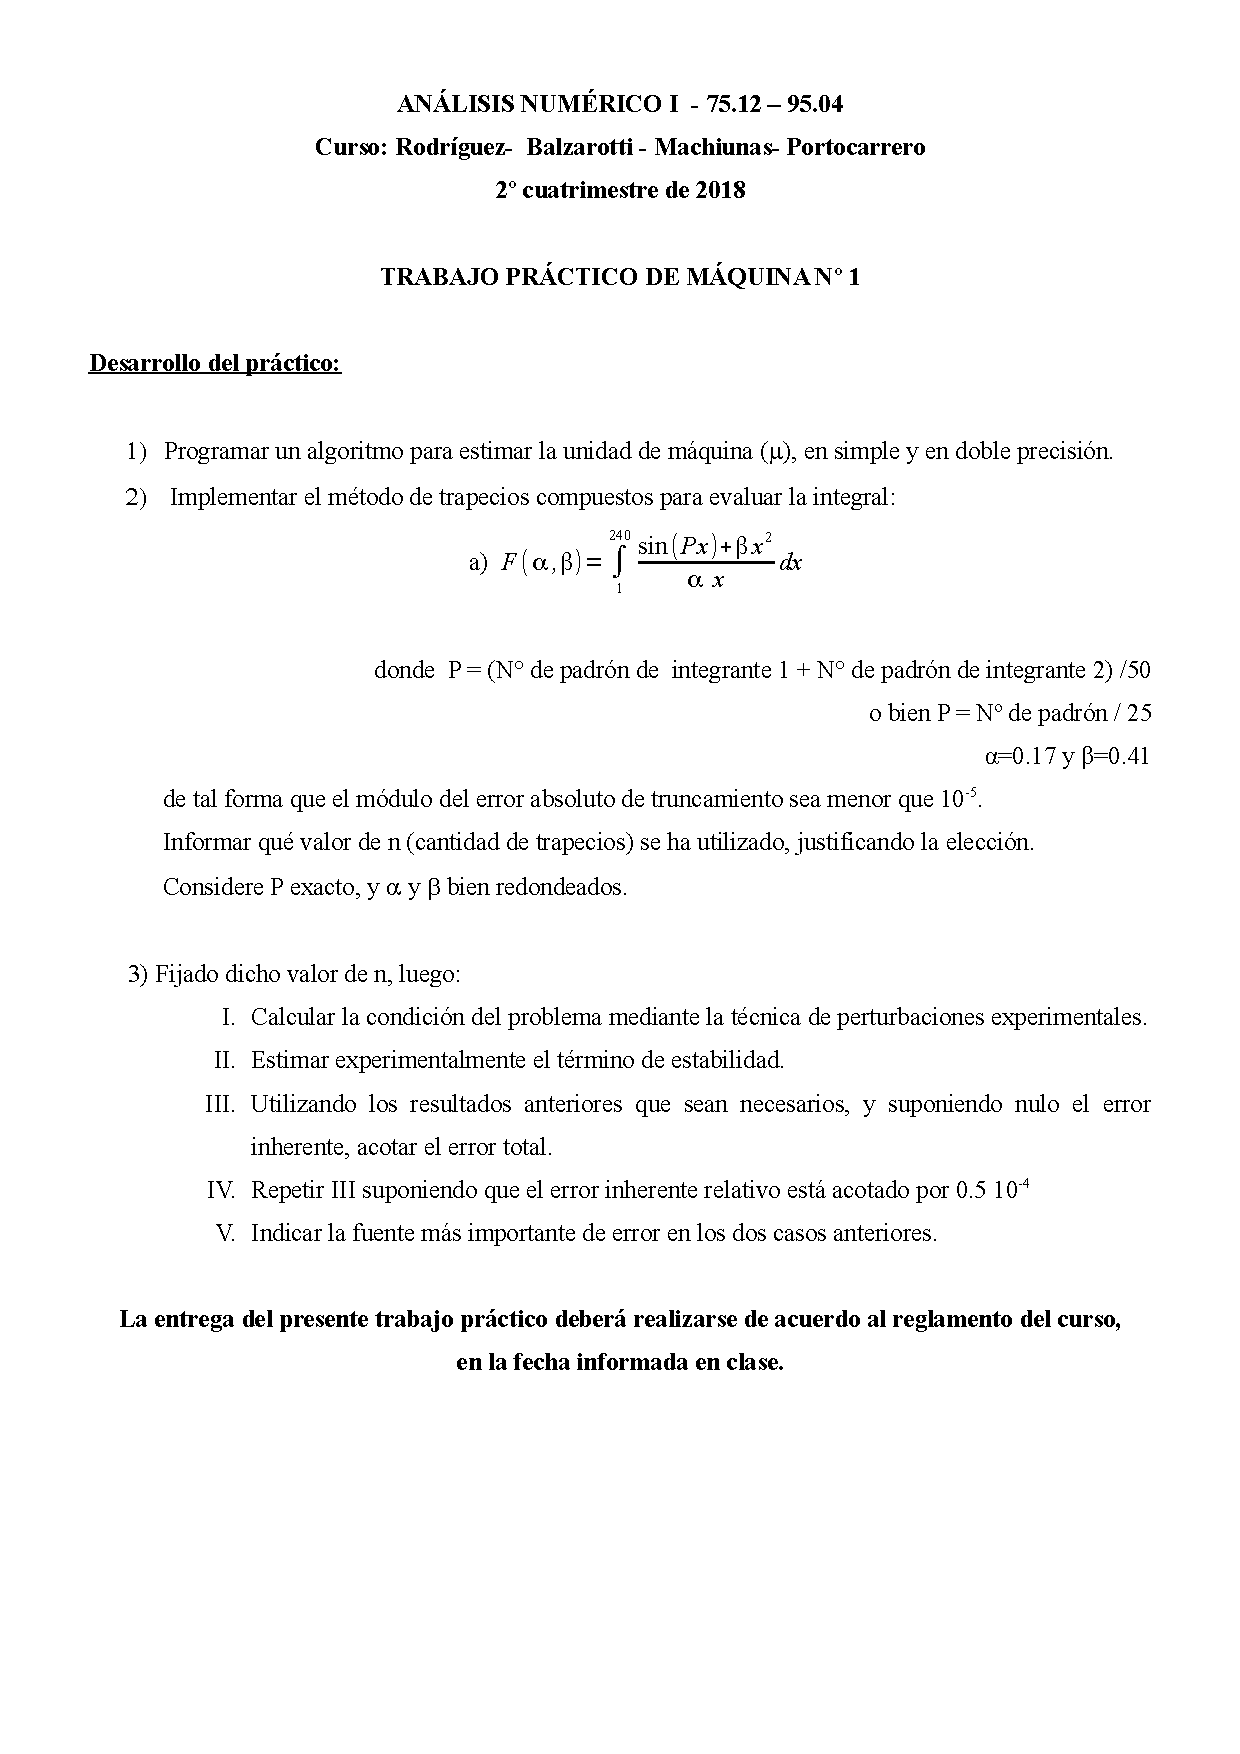
\includepdf[pages=-,pagecommand={\thispagestyle{enunciado}}]{TP1-Enunciado.pdf}

\pagenumbering{gobble}
\tableofcontents
\thispagestyle{onlyheader}
\newpage


\pagenumbering{arabic}
\setcounter{page}{1}

\section{Introducción}
Introducción, que incluya los objetivos específicos del TP, puede incluir descripción del
problema concreto a resolver y mencionar los métodos específicos empleados y un resumen del
trabajo (1 página máximo; no incluir explicaciones teóricas en esta sección, ni generalidades
sobre el cálculo numérico).

\section{Desarrollo}
Para los cálculos del \(\mu\) se utilizó el algoritmo del ejemplo 6.4 del libro de Hernan Gonzales \cite{Gonzales}.
 
 Desarrollo del trabajo (en esta sección explicarán cómo emplearon/adaptaron los
resultados teóricos ya dados en clase para resolver el problema numérico particular, y cómo
salvaron dificultades halladas en la implementación; emplearán el editor de ecuaciones -o
similar- para las fórmulas que mencione; centrando las fórmulas y numerándolas). La
bibliografía consultada debe estar referenciada en la sección correspondiente. El código
resultante no va en el desarrollo, sino que se colocará en el Anexo I.

\section{Resultados}
 Resultados: se espera un resumen que permita observar de forma clara y sencilla los
resultados obtenidos desde que se procede a ejecutar el código. Cuando corresponda, se
incluirán figuras (realizadas con Octave o Matlab) y breves tablas.

\section{Conclusiones}
 Conclusiones, que incluyan el análisis y la discusión (específica) de los resultados.

\newpage
\appendix
\section{Anexo I: Código Fuente}

\lstinputlisting[language=Octave]{mu_simple.m}
\lstinputlisting[language=Octave]{mu_doble.m}

Anexo I: código fuente impreso (obligatorio) realizado en Octave o Matlab de todos los
archivos .m empleados. Citar el sofware y versión empleados, así como el equipo usado para
ejecutarlo. (de emplear Octave, procurar mantener el código compatible con Matlab,
procediendo como se explicó en clase, por ejemplo: uso de end en vez de endif, endfor...;
definición de funciones con el comando function en un archivo .m y no usando @, etc.).

\section{Anexo II: Resultados Numéricos}
\begin{lstlisting}[language=Octave]
>> mu_simple
mu =    1.0000e-08
>> mu_doble
mu =    1.0000e-16
\end{lstlisting}

Anexo II: Resultados numéricos completos obtenidos al correr el programa (máximo 5
hojas). Acá colocar las tablas completas de resultados, de ser pertinente.

\section{Anexo III: Información Adicional}
Anexo III: Otra información relevante, por ejemplo, comentarios sobre las deducciones
teóricas de las fórmulas, o explicación de comandos de Octave o Matlab empleados que no
fueron explicados en clase, o del contexto o aplicación (opcional) (máximo 2 hojas)

\newpage

\phantomsection 
\addcontentsline{toc}{section}{Bibliografía}
\renewcommand\refname{Bibliografía}
\begin{thebibliography}{9}

\bibitem{Gonzales} 
Gonzales, Hernan: 
\textit{Análisis Numérico, Primer Curso}
Buenos Aires: Nueva Librería, 2002.

\end{thebibliography}
\end{document}

